\documentclass[submit,techrep,noauthor]{ipsj}

% \usepackage[dvips]{graphicx}
\usepackage[dvips,dvipdfmx]{graphicx}
\usepackage{url}
% \usepackage{graphicx}
% \usepackage[dvipdfmx]{color}
\usepackage{caption}
\usepackage{tabularx}
\newcolumntype{Y}{>{\arraybackslash}X}
\usepackage{latexsym}
% \usepackage{hyperref}

\usepackage{listings,jlisting}
\lstset{
  basicstyle={\ttfamily},
  identifierstyle={\small},
  commentstyle={\textit},
  keywordstyle={\small\bfseries},
  ndkeywordstyle={\small},
  stringstyle={\small\ttfamily},
  frame={tb},
  breaklines=true,
  columns=[l]{fullflexible},
  numbers=left,
  xrightmargin=0zw,
  xleftmargin=1zw,
  numberstyle={\scriptsize},
  stepnumber=1,
  numbersep=1zw,
  lineskip=-0.5ex
}
\renewcommand{\lstlistingname}{ソースコード}
\newcommand{\lstref}[1]{ソースコード\ref{#1}}

\begin{document}

\affiliate{cs}{筑波大学大学院理工情報生命学術院システム情報工学研究群情報理工学位プログラム}
\affiliate{ccs}{筑波大学計算科学研究センター}

\title{CA VOL: HDF5におけるコンテキストによるI/O最適化}

\author{木下 嵩裕}{Kinoshita Takahiro}{CS}[kinoshita@hpcs.cs.tsukuba.ac.jp]
\author{建部 修見}{Osamu Tatebe}{CCS}[tatebe@cs.tsukuba.ac.jp]

\begin{abstract}
	HPCにおけるアプリケーションの多くはHDF5やnetCDF等の高レベルI/Oライブラリを利用してI/O処理を行う.
	HDF5には,Virtual Object Layer(VOL)という機能があり,高レベルなAPIでI/O処理を置き換える仕組みがある.
	既存のI/Oでは,このVOLの中で利用可能であるデータの型のサイズ,データのレイアウト等のコンテキストを活用できていない.
	本研究では,このVOLで得ることのできるコンテキストを活用することで,I/O処理の最適化を行うVOLプラグインCA VOLを提案する.
	コンテキストを元にデータの書き込み境界とファイルシステムでのチャンクサイズを合わせ,I/Oの並列度を高めることで,I/Oを高速化した.
\end{abstract}

\maketitle

\section{はじめに}
近年,HPCでは,計算機の性能が指数関数的に向上している.
しかし,演算器の性能向上と比較して,ストレージの性能向上は計算機の性能向上に追いついていない.
特に,近年のシミュレーションサイズの増加に伴い,ストレージ性能の不足がシステムのボトルネックとなっている.
このストレージとの性能の乖離へ対処するために,
ストレージ中間層を導入し,グローバルファイルシステムへの書き込みを高速化する研究\cite{wang2016burstbuffer,moody2017unifyfs},
ジョブ中で一時的にデータを格納するad-hocファイルシステム\cite{vef2018gekkofs,tatebe2022chfs}の研究がされてきた.
キャッシュストレージ層,新しいストレージデバイスが登場することにより,
ストレージレイヤーはより複雑になっている.
このような複雑なストレージレイヤーやデバイスの特性を意識することなく
効率的にアプリケーションを実行できることが求められている.

多くのHPCアプリケーションは,HDF5\cite{hdf5}やpnetCDF\cite{pnetcdf}等高レベルI/Oライブラリを利用してI/O処理を行う\cite{byna2020exahdf5}.
これらの高レベルI/Oライブラリでは,内部のI/O処理に,MPI-IOと言われるライブラリが利用されている.
MPI-IOにはIOを抽象化する仕組みがあり,そこで,Lustreなどそれぞれのファイルシステムに対してのコネクターが実装される.
HDF5等のライブラリでは,そのコネクター経由で各グローバルファイルシステムに対して書き込みを行っている.
特定のサイズの大量データの連続書き込みにおいては高速だが,
特定のアクセスパターン,例えば,小規模でスパースな書き込み,特定のサイズ以外のstridedアクセス,ランダムアクセスが多い場合,その性能は著しく低下する.
HDF5には,高レベルなAPIでI/Oの機能の入れ替えが可能となるVirtual Object Layer(VOL)という機能がある.
このVOLを活用したI/O処理について研究が進められている\cite{zheng2022hdf5,tang2021transparent,soumagne2021accelerating}.
VOLはその実装でデータの型のサイズ,データのレイアウト等の情報,コンテキストを得ることができる.
これらの研究では,VOLの実装で得ることのできる様々な情報を活用していない.
このVOLで得られるコンテキストを活用することで,I/O処理の高速化が期待される.

Lustre\cite{Lustre},CHFS\cite{tatebe2022chfs}といったファイルシステムではファイルをあるサイズのオブジェクトに分割して保存する.
一貫性を確保するために,そのオブジェクトごとにロックを取る.そのため,同一のオブジェクトに対する書き込みはロックを取られ,順番に行われる.
そのオブジェクトのサイズは,stripe\_sizeやchunk\_sizeと呼ばれるパラメータで指定される.
そのパラーメータで指定されたオブジェクトのサイズと書き込みサイズがあっていない場合,
1つのオブジェクトに対して複数のプロセスから同時に書き込み要求が行われることになる.
しかし,ロックをとるため,その書き込みは順番に行われ,並列度が失われるという問題がある.
また,HDF5などのライブラリによるファイル書き込みでは,
書き込み粒度とそのオブジェクトのサイズを合わせたとしても,その境界に必ずしもアライメントされるわけではないため,
プロセス間での書き込み競合を減らすことが難しい.

本研究では,これまで活用されてこなかった,HDF5のVirtual Object Layerで得ることのできるコンテキストを活用することで,
各プロセスのデータ書き込み境界とストレージのチャンクサイズを合わせることにより並列度を高め,I/Oを高速化するVOLプラグインCA VOLを提案する.
これにより,自動的にチャンクサイズ等を決定し,プロセスどうしのI/O競合を抑え並列度を高めることができる.


本研究の貢献は以下の通りである.
\begin{itemize}
	\item HDF5で得られるコンテキストを利用してI/Oの高速化に活用するVOLプラグインの設計.
	\item 性能評価によりコンテキストを利用することによるI/Oの高速化を示す.
\end{itemize}


\section{関連研究}

HDF5のVOLを用いたI/O処理についての研究は,
CacheVOL\cite{zheng2022hdf5}やDAOS VOL\cite{soumagne2021accelerating},Async VOL\cite{tang2021transparent}がある.

Huihuo Zengらによる計算ノードのローカルSSDを利用した研究Cache VOL\cite{zheng2022hdf5}
では書き込み時には,まず各ノードのノードローカルSSDに一時的に書き込み,
その後,非同期で共有ファイルシステムに書き戻す.
プログラムから見える実効速度はノードローカルSSDの速度のノード数倍のものになり,
スケーラブルで高速なI/Oの実現が可能である.
この研究では,単純に自ノードが発行したI/Oをノードローカルストレージに一時的に書き込み,それを非同期に書き戻すのみであり,
HDF5のVOL中で得ることができるコンテキストを活用できていない.

Jerome Sounmagneらによる分散オブジェクトストレージであるDAOS\cite{Breitenfeld2017DAOSFE}を使ったDAOS VOL\cite{soumagne2021accelerating}がある.
DAOSは分散オブジェクトストレージであり,高いスケーラビリティを持つことが特徴である.
この研究では,HDF5のVOLのレイヤーの機能を1つのオブジェクトに対応させ,DAOSに格納している.
特に,Datasetの書き込みの際にはストライピングが可能であり,そのスライピング数をプログラム中でH5D\_set\_chunk()関数によってユーザーが設定できる.
しかし,この研究では,VOLの実装中で得られるコンテキストをベースに自動で設定できない.

\section{設計}
\subsection{Virtual Object Layer/Virtual File Driver}
\begin{figure}[t]
	\centering
	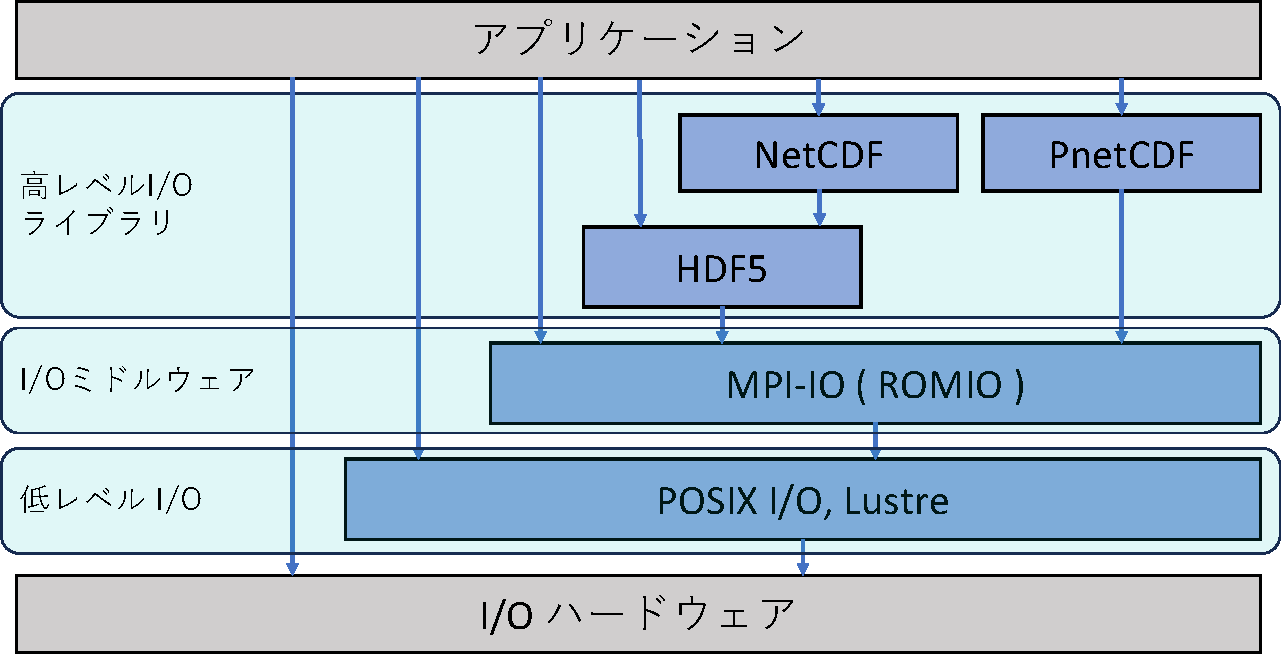
\includegraphics[page=1,width=\linewidth]{figure-crop.pdf}
	\caption{HPCのIOスタック}
	\label{fig:iotstack}
\end{figure}

HPCにおけるI/Oスタックについて示した図を\figref{fig:iotstack}に示す.
アプリケーションは,低レベルなAPIを直接使うこともできるが,高レベルI/Oライブラリ経由してデータの書き込みを行うことが多い.
NetCDFやHDF5といったライブラリ経由で何らかのデータを書き込みを行ったとき,そのライブラリは内部でI/Oミドルウェアを利用しI/Oを行う.
次に,HDF5のI/Oスタックについて示した図を\figref{fig:hdf5stack}に示す.
高レベルIOライブラリは内部的には低レベルI/Oライブラリを利用している.
HDF5のAPIで何らかの書き込みが行われたとき,低レベルI/Oライブラリに至るまでに,
HDF5のAPIを抽象化するVirtual Object Layerと
ファイルシステムに対しての操作をするVirtual File Driverという2つのレイヤーを経由する.

まず,Virtual Obejct Layerについて説明する.
HDF5は1つのファイルに任意のデータ型の配列を保存したり,
複数のデータ型の配列をまとめて保存したりできる.
HDF5の実際にユーザーから見える機能をそのまま抽象化できる仕組みがVOLである.
HDF5の機能,Dataset,Group,Attribute,Datatype,File等の機能ごとに,
open,create,read,write,closeといった関数コールバックを定義することで独自の処理を行うことができる.
特にDatasetのcallbackの定義を\lstref{lst:volcallback}に示す.
\begin{lstlisting}[caption=VOLのDataset Callbackの定義,label=lst:volcallback,language=c]
static void *H5VL_dataset_create(void *obj, const H5VL_loc_params_t *loc_params, const char *name, hid_t lcpl_id, hid_t type_id, hid_t space_id, hid_t dcpl_id, hid_t dapl_id, hid_t dxpl_id, void **req);
static void *H5VL_dataset_open(void *obj, const H5VL_loc_params_t *loc_params, const char *name, hid_t dapl_id, hid_t dxpl_id, void **req);
static herr_t H5VL_dataset_read(size_t count, void *dset[], hid_t mem_type_id[], hid_t mem_space_id[], hid_t file_space_id[], hid_t plist_id, void *buf[], void **req);
static herr_t H5VL_dataset_write(size_t count, void *dset[], hid_t mem_type_id[], hid_t mem_space_id[], hid_t file_space_id[], hid_t plist_id, const void *buf[], void **req);
static herr_t H5VL_dataset_get(void *dset, H5VL_dataset_get_args_t *args, hid_t dxpl_id, void **req);
static herr_t H5VL_dataset_specific(void *obj, H5VL_dataset_specific_args_t *args, hid_t dxpl_id, void **req);
static herr_t H5VL_dataset_optional(void *obj, H5VL_optional_args_t *args, hid_t dxpl_id, void **req);
static herr_t H5VL_dataset_close(void *dset, hid_t dxpl_id, void **req);
\end{lstlisting}
既存の実装としては.Native VOL,Async VOL,DAOS VOL,Cache VOLなどがある.
通常のHDF5のファイルの読み書きに関してもNative VOLプラグインで実装がされ,すべてのI/OがこのVOLを経由して行われる.
このVOLでは,高レベルなAPIでインターセプトするため,DAOS VOLのように別のストレージシステムに書き込むこともできる.
また,Cache VOLのように,ノードローカルSSDに一時的に書き込みを行い,既存のNative VOLを利用し非同期に書き込むを行う
パススルータイプのプラグインも実装できる.

Virtual File Driver(VFD)について説明する.
Virtual Obejct Layer実装であるNative VOL等で使われているHDF5の内部APIによって行われた操作を,
実際のI/Oに変換するレイヤーである.
例えば,Datasetに対して何らかのデータを書き込んだとき,Native VOLから,
H5D\_\_write()という関数が呼ばれる.
まず,この操作がHDF5の実装によって,ファイルのどの位置からどの位置までの書き込みであるかという操作に変換される.
その操作を実際にファイルシステムに対して行うのがVirtual File Driverである.
実装としては,POSIX,MPI-IOなどがある.
VOLと同様にopen,close等の関数コールバックを実装することで独自のI/O処理を行うことができる.
writeコールバックではPOSIX I/Oと似たようなインターフェースになっており,ファイルディスクリプタのように使える
構造体へのポインターとファイルでのoffsetと書き込みサイズが渡され,それによってプラグインが書き込みを行う.
HDF5では,このVFDでMPI-IO向けの実装がされており,
環境変数を指定することによって,MPI-IOを使ってファイルに対して書き込みを行うことができるようになっている.

VFDプラグインとVOLプラグインについて共有ライブラリとしてビルドし,.soファイルのあるディレクトリを
環境変数に設定し,HDF5のAPIを利用するアプリケーションから簡単に利用できる.
ソースコード\ref{lst:plugin}にプラグインを利用する方法を示す.
\begin{lstlisting}[caption=プラグインの利用方法, label=lst:plugin]
HDF5 PLUGIN PATH=/path/to/plugin/directory HDF5 VOL CONNECTOR=”{my vol connector under vol=0;under info=}” ./program
\end{lstlisting}
このように環境変数を指定するだけで,独自のI/O処理に切り替えることができる.
MPI-IOにて新しいコネクターの実装をしたときは,MPI全体をビルドし直す必要があるため,
アプリケーションユーザーからの利用にハードルがあった.
この点,HDF5のVOLとVFDは
環境変数を指定するのみで実行可能であり,
ポータビリティに優れ,アプリケーションへの適用が容易である.


\begin{figure}[t]
	\centering
	\includegraphics[page=7,width=\linewidth]{figure-crop.pdf}
	\caption{HDF5のIOスタック}
	\label{fig:hdf5stack}
\end{figure}


\subsection{HDF5のファイル構造}
HDF5のファイル構造について説明する.
HDF5では単一の大きなファイルに対して,複数のデータセット,グループ,属性,データ型等を格納できる.
HDF5のファイルの中での各データの配置のされ方,特にDatasetについて示した図を\figref{fig:hdf5file}に示す.
Datasetを書き込んだ際は,Dataset headerとDataset dataに分けてファイルに格納される.
Dataset headerには,データの型やデータのレイアウトや格納のされ方を示すDataspaceなど,Datasetに関するメタデータが格納される.
Dataset dataには,Dataset headerで表されたデータの実データが格納される.

次に,HDF5にデータを格納するときの変換のされ方について説明する.
HDF5のデータをファイルに格納する際は,多次元のメモリの配列を1次元に展開して格納する,
特に2次元でメモリ上にあるデータをファイルに書き込むときの様子を示した図を\figref{fig:hdf5mem2file}に示す.
図のように,データのインデックスが若いものから順番に展開してDataset dataに書き込まれる.

\begin{figure}[t]
	\centering
	\includegraphics[page=13,width=\linewidth]{figure-crop.pdf}
	\caption{HDF5のファイルの中での各データの配置のされ方}
	\label{fig:hdf5file}
\end{figure}

\begin{figure}[t]
	\centering
	\includegraphics[page=17,width=\linewidth]{figure-crop.pdf}
	\caption{HDF5にデータを格納するときの変換のされ方}
	\label{fig:hdf5mem2file}
\end{figure}


\subsection{Virtual Object Layerで得られる情報}
VOLのDatasetのCallbackでは,Datasetの書き込みに関しての情報を得ることができる.
その情報について表した図を\figref{fig:hdf5infoinvol}に示す.


\begin{figure}[t]
	\centering
	\includegraphics[page=16,width=\linewidth]{figure-crop.pdf}
	\caption{HDF5のVOLのdataset\_writeで得られる情報}
	\label{fig:hdf5infoinvol}
\end{figure}
\subsection{設計}


HDF5経由で呼び出された際に,VOLの機能を利用する.
そのとき,Datasetへの書き込みに関してのみ,
その書き込み時に得られるコンテキストをもとに,CHFSに対しての書き込みを行う.
また,Dataset以外の書き込みをNative VOLに渡す.
このようにすることで,Datasetの書き込みに関してのみ,
CHFSに対してオフローディングされる.
それ以外の書き込み関しては従来どおり,Native VOLによって処理され,
MPI-IO経由でファイルシステムに対して書き込みを行う.

Datasetのみの書き込みをCHFSに対して行ったことについて説明する.
Datasetの実データ以外の書き込み,
例えばデータセットに付随するレイアウト情報などを扱おうとすると,
HDF5の膨大な仕様を把握し,そのオプション1つ1つに対して対応しなければならない.
そのため,本実装では,Datasetの実データのみコンテキストに基づいて
CHFSに対して書き込みを行うこととした.
なお,シミュレーションサイズが増加するのに対して,
増加するのはメタデータの書き込みではない.
あるシミュレーションデータの状態を保存しようとしたとき,
メタデータはそのあるデータの塊1つに対して1つしか書き込まれない.
シミュレーションサイズが増加する際に増加するのは,その問題のサイズであり,メタデータの量ではない.
つまり,メタデータの書き込みはシミュレーションサイズの増加に対して増加しない.
シミュレーションサイズが大きくなるにつれボトルネックとなるのは,
Datasetの実データの書き込みである.
そのため,本実装ではDatasetの実データのみを
コンテキストに基づいた書き込みを行うこととした.
提案手法について示した図を\figref{fig:dividevol}に示す.
Datasetの実データのみ,

Lustreやchfsではオブジェクト,チャンク単位での並列性がない.
同じチャンクに対して複数のプロセスから書き込みが行われると,その書き込みは順番に行われ並列度が失われる.
そのため,書き込みサイズとチャンクサイズ/ストライプサイズがあっていることが重要となってくる.
4000 x 4000のデータセットを書き込むときの例を図に示す.
書き込みのサイズがチャンクサイズとあっていないIOパターンの図を\figref{fig:wrongio}に
書き込みのサイズがチャンクサイズとあっているIOパターンの図を\figref{fig:correctio}に示す.
書き込みサイズがチャンクサイズとあっていない場合,この例では,
131プロセスから同じチャンクに対して書き込みが行われている.
書き込みサイズがチャンクサイズとあっている場合では,各チャンクに対して
1プロセスからの書き込みが行われている.
このように,書き込みサイズとチャンクサイズがあっていない場合,
同じチャンクに対して複数のプロセスから書き込みが行われるため,
その書き込みは順番に行われ並列度が失われる.
なおLustreでは2MiB以下のstripe\_sizeでは2MiBでアライメントされてしまうので,
2MiB以下のサイズにしてもパフォーマンスが出ない.
しかし,CHFSでは2MiB以下のサイズに関しても設定可能であり,
このチャンクサイズと書き込みサイズを合わせることで
並列度を高めることが可能であるため,大きなパフォーマンスの向上が見込まれる.

\begin{figure}[t]
	\centering
	\includegraphics[page=14,width=\linewidth]{figure-crop.pdf}
	\caption{書き込みサイズとチャンクサイズがあっていないIOパターン}
	\label{fig:wrongio}
\end{figure}

\begin{figure}[t]
	\centering
	\includegraphics[page=15,width=\linewidth]{figure-crop.pdf}
	\caption{書き込みサイズとチャンクサイズがあっていないIOパターン}
	\label{fig:correctio}
\end{figure}

\begin{figure}[t]
	\centering
	\includegraphics[page=8,width=\linewidth]{figure-crop.pdf}
	\caption{今回の提案手法CA VOLの構成}
	\label{fig:dividevol}
\end{figure}

\section{実装}

HDF5を経由してdatasetを書き込む際,
必ずしもdatasetの書き込みの粒度とLustre等のファイルシステムのチャンクサイズが一致するとは限らない.
そのため,datasetの書き込みサイズに基づいてチャンクサイズを決定するような方法を提案する.
その書き込みのプロセスの疑似コードをソースコード\ref{lst:chunksize}に示す.
rankが0のプロセスがチャンクサイズを決定し,そのチャンクサイズでファイルを作成する.
それを待ち,各プロセスが書き込みを行う.

多くのアプリケーションでは各プロセスが担当する領域は何らかの規則に従い等しく割り当てられることが多い.
つまり,すべてのプロセスが同様の粒度でデータを書き込むことが多くなる.

\begin{lstlisting}[caption=チャンクサイズの決定,label=lst:chunksize]
function dataset_write(params)
  if rank == 0 {
    chunk_size = calc_dataset_write_size(params)
    chfs_create_with_chunk_size(set_chunk_size(chunk_size))
	}
  MPI_Barrier()

  fd = chfs_open()
  chfs_pwrite(fd, params)
end
\end{lstlisting}




\section{評価}
\subsection{評価環境}
提案手法の実装に関して性能を評価する実験をした.
実験には筑波大学のスーパーコンピューター\cite{ccs2022pegasus}を使用した.
Pegasusの構成を表\ref{tab:pegasus}に示す.
また,計算機クラスターに接続されている並列分散ファイルシステム,Lustreのスペックを
表\ref{tab:lustre}に示す.

% textlint-disable
\begin{table}[t]
	\caption{Pegasusのスペック}
	\label{tab:pegasus}
	\centering
	
	\begin{tabularx}{\linewidth}{Y|Y}
		\hline \hline
		CPU    & Intel Xeon Platinum 8468 (codenamed Sapphire Rapids) 2.1GHz/48c \\ \hline
		GPU    & NVIDIA H100 Tensor Core GPU with PCIe                           \\ \hline
		メモリ    & 128GiB DDR5-4800                                                \\ \hline
		不揮発メモリ & 2TiB Intel Optane persistent memory 300 series                  \\ \hline
		SSD    & 2 x 3.2TB NVMe SSD (7 GB/s)                                     \\ \hline
		ネットワーク & NVIDIA Quantum-2 InfiniBand platform (200 Gbps)                 \\ \hline
	\end{tabularx}
\end{table}

\begin{table}[t]
	\caption{Lustreのスペック}
	\label{tab:lustre}
	\centering
	
	\begin{tabularx}{\linewidth}{Y||Y}
		\hline \hline
		ファイルシステム & DDN EXAScaler Lustre                                          \\ \hline
		MDS/MDT  & 1.92 TB NVMe SSD x 11 ( 8D + 2P + 1HS)                        \\ \hline
		OSS/OST  & 18 TB 7200rpm NL-SAS x 534 (( 33 drives 8 pools + 3HS ) * 2 ) \\ \hline
	\end{tabularx}
\end{table}

\subsection{実験方法}
素粒子物理シミュレーションのI/Oパターンを模したI/Oベンチマークh5bench\cite{h5bench}を利用して評価した.
チェックポインティングのI/Oパターンを模したものであり,各stepで設定した問題サイズのDatasetを8つ作成し,書き込む.
問題サイズは$8192 \times 8192$,timestep数は3に設定した.各ノードに16プロセスを配置し,ノード数を1-64ノードまで変化させた.
h5benchの書き込みのアクセスパターンにはsegmentedであるが,stridedなアクセスパターンについても,
実データの書き込み部分でstridedに変換して評価を行った.
また,今回の実装では,コンテキストに基づきchunk sizeを決定することで,ファイルシステムでのデータ境界と
データの書き込み境界を合わせることにより,I/Oの並列度を高めることを目標としていた.
それと比較するために,
今回の実験では,そのチャンクサイズを512KiBに固定して書き込みを行ったものについても最適化なしとして測定を行った.

\subsection{CA VOLのstridedアクセスパターンに対する性能評価}
CA VOLのstridedアクセスパターンのときのバンド幅を比較する.
その結果を\figref{fig:h5writestrided}に示す.
コンテキストよりCA VOLによってチャンクサイズは64KiBに自動的に設定された.
バンド幅は64ノードまでスケールしており,64ノードでは最適化によって約1.5倍の性能向上が見られた.
最適化なしでは512KiBで書き込みを行っているが,
それぞれのチャンクには4プロセスから同時に書き込みを行うことになるため,並列度が落ち,
ハンド幅が低下したと考えられる.

stridedなアクセスパターンにおいて,データの書き込みとストレージの境界を合わせることにより,
より効率的なI/Oが行われることが確認できた.

\begin{figure}[t]
	\centering
	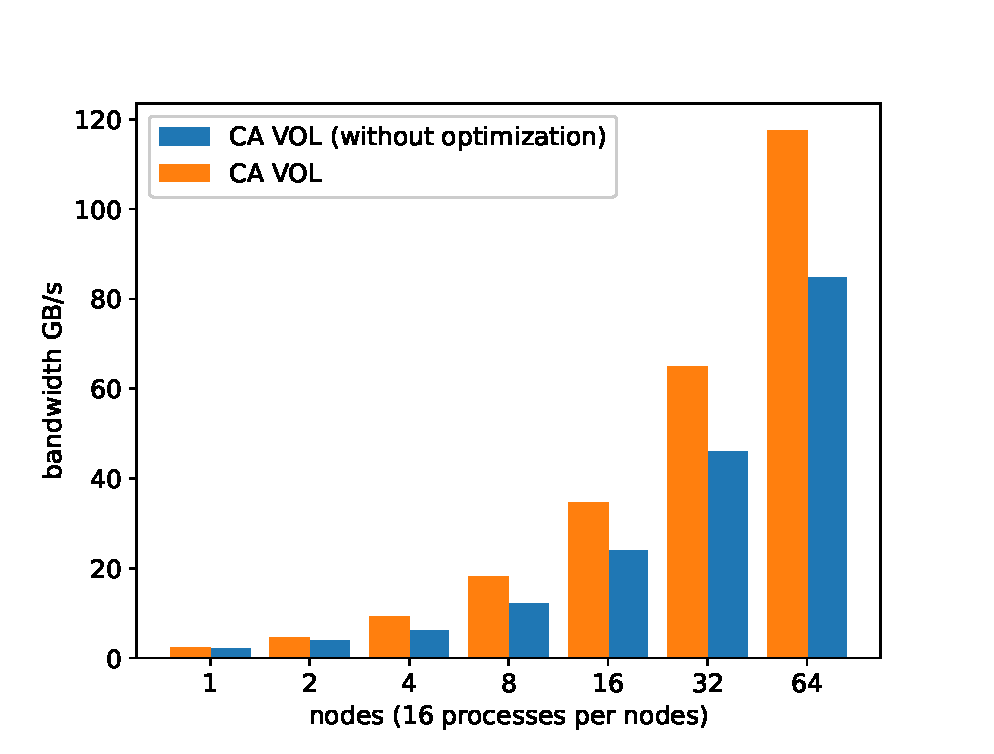
\includegraphics[width=\linewidth]{figure/chfs_strided.eps}
	\caption{h5bench write 問題サイズ$8192 \times 8192$,stridedアクセスパターン,ノード数を1から64まで変化させたときのCA VOLのバンド幅}
	\label{fig:h5writestrided}
\end{figure}

\subsection{CA VOLのsegmentedアクセスパターンに対する性能評価}

\begin{figure}[t]
	\centering
	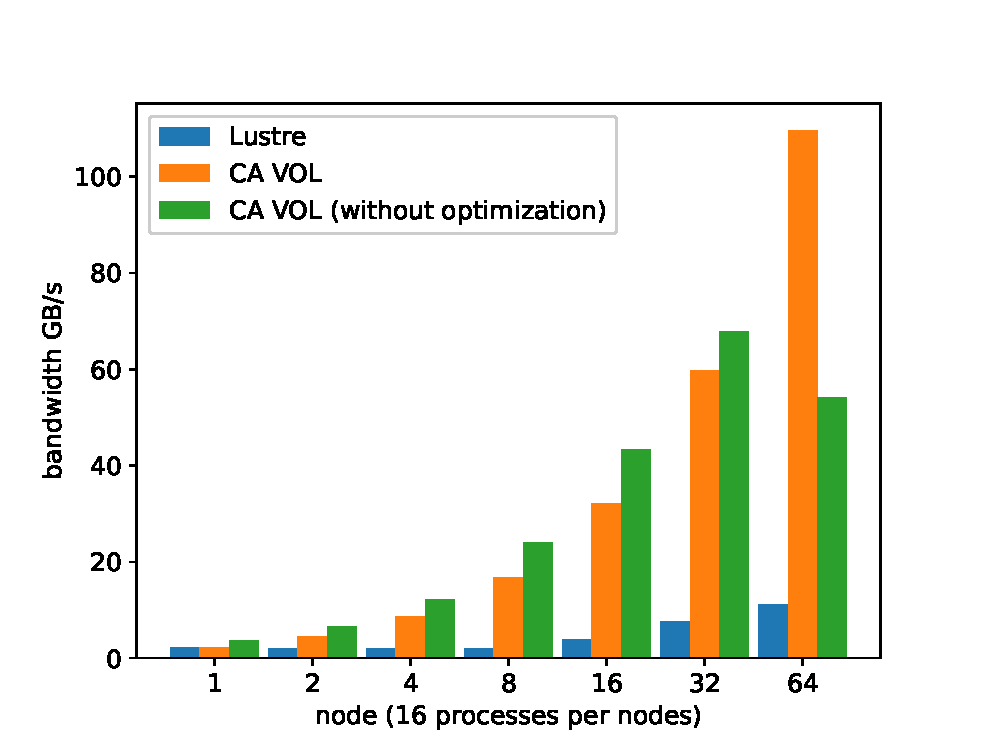
\includegraphics[width=\linewidth]{figure/segmented_chfs.eps}
	\caption{h5bench write 問題サイズ$8192 \times 8192$,segmentedアクセスパターン,ノード数を1から64まで変化させたときのCA VOLのバンド幅}
	\label{fig:h5writesegmented}
\end{figure}


CA VOLのsegmentedアクセスパターンのときのバンド幅を比較する.
その結果を\figref{fig:h5writesegmented}に示す.
CA VOLのバンド幅は64ノードまでスケールしており,64ノードではCA VOLのバンド幅がLustreのバンド幅の約10倍程度となっている.
512KiB固定チャンクサイズのときは1-32ノードではスケールしているが,64ノードではスケールしなくなっている.
1-32ノードに関して,最適化なしのCA VOLのほうがバンド幅が大きいが,これは,
最適化なしのほうではチャンクを小さく分割しているため,多くのノードに対して分散して書き込みが行われていたためだと考えられる.
しかし,64ノードでは最適化なしのほうがバンド幅が低下している.
これは,領域を小さく分割しすぎたため,RPCによるオーバーヘッドが増加したためだと考えられる.

\section{まとめ}
本研究では,計算性能の飛躍的な向上に対してI/O性能が追いついていない問題に対して,
高レベルI/Oライブラリで得ることのできる書き込みコンテキストを利用することによるI/Oの高速化
の可能性を示した.

高レベルI/Oライブラリ経由で書き込まれるデータの粒度と
ストレージの最下層の操作単位であるオブジェクトのサイズ,チャンクサイズやストライプサイズは一致していないことが多い.
また,仮にデータの書き込みの粒度とチャンクサイズ等が等しくても,
ファイルの中でのデータの配置のアライメントの関係で,複数のプロセスから同時に同じ領域に書き込んでしまい.
その部分での並列度が失われる.
アプリケーションユーザーはこのような低層のストレージの特性を意識することなく,
高いI/O性能を得ることが望ましい.

高レベルI/Oライブラリでの抽象化レイヤー,VOLにおいて得ることのできる
レイアウト情報などのコンテキストを利用し.
そのデータセットの書き込みに対して最適なチャンクサイズを決定することで,書き込みの高速化を確認した.

ストレージ階層が複雑化し,その各ストレージの性能を最大限活かすためには,
このような高レベルI/Oライブラリで得ることのできる書き込みコンテキストを活用することが重要である.


\begin{acknowledgment}
	本研究の一部は,JSPS科研費22H00509,
	国立研究開発法人新エネルギー・産業技術総合開発機構(NEDO)
	「ポスト5G情報通信システム基盤強化研究開発事業」(JPNP20017)委託事業,
	文部科学省「次世代計算基盤に係る調査研究」事業,
	筑波大学計算科学研究センター学際共同利用プログラム,
	および富士通との特別共同研究の結果得られたものです.
\end{acknowledgment}

\bibliographystyle{ipsjsort}
\bibliography{references}

\end{document}
